\documentclass{article}
\usepackage{graphicx} % Required for inserting images
\usepackage{algorithm}
\usepackage{algpseudocode}



\title{Final Labwork Advanced Programming for HPC}
\author{Ta Quang Hieu - M22ICT002}
\date{November 2023}

\begin{document}
	
	\maketitle
	
	\section{The problem}
	This project concerns image contrast enhancement using some histogram equalization techniques. During this project, I will implement various methods on the GPU to solve this problem, using the following techniques :
	
	\begin{itemize}
		\item HE: classical Histogram Equalization.
		\item AHE: Adjusted Histogram Equalization.
		\item WHE: Weighted Histogram Equalization.
		\item EIHE.
		\item MMSICHE.
		\item CLAHE: Contrast Local Adaptive Histogram Equalization.
		\item ACLAHE: Automatic Contrast Local Adaptive Histogram Equalization.
	\end{itemize}    
	
	To study the efficiency of the algorithms, I will use two different metrics:
	\begin{itemize}
		\item AME which is the sum of the absolute value of the difference per pixel. This is a reduction made from the transformation of two images.
		\item Entropy: it relies on the global histogram of the image.
	\end{itemize} 
	
	\section{Introduction}
	
	During the project week, because I have some issues in my family - as I have emailed you before - so during this week I need to do the project for both parts of this course Dr. Son part, and also yours. This makes me unable to finish all the other parts but I have tried my best with this project. In this project, I have done the implementation of HE, AHE and EIHE algorithm, I also tried to finish WHE but I don't understand it, for MMSICHE, CLAHE and ACLAHE, I haven't been able to read them. For the original image that I use, please take a look at Figure~\ref{fig:original}.
	
	\begin{figure}
		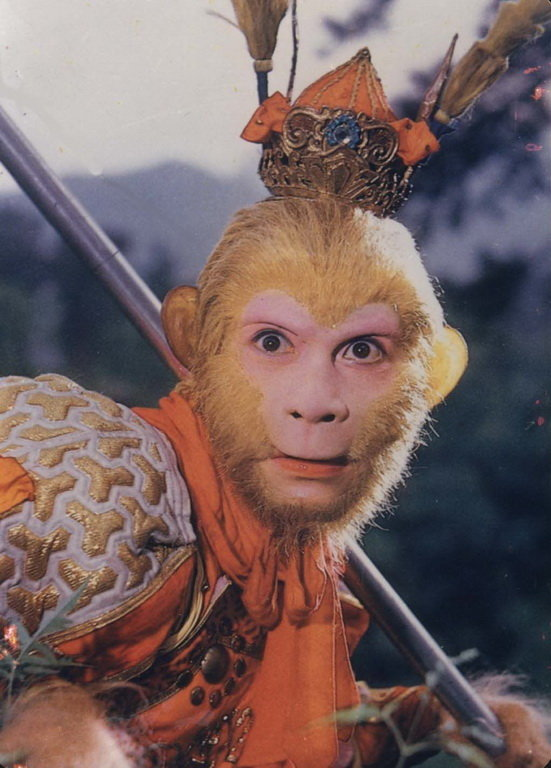
\includegraphics[width=\linewidth]{img/original.png}
		\caption{The original image.}
		\label{fig:original}
	\end{figure}
	
	\section{The general steps}
	
	The general steps of these Histogram Equalization algorithms are listed below:
	
	\begin{itemize}
		\item Convert the image from RGB to HSV and we will modify the V channel
		\item Calculate the histogram (and the modified histogram - if not the original HE) for the V channel
		\item Calculate the CDF from the histogram
		\item Mapping each pixel from the original image based on the CDF
	\end{itemize}
	
	\section{Implementing Histogram Equalization algorithms}
	
	\subsection{Convert the image from RGB to HSV}
	
	After loading the image, I will use a function to convert the image from RGB to HSV in order to use the V channel for calculating the histogram.
	
	This is the function that I used to turn the image from RGB to HSV.
	
	\begin{verbatim}
		from numba.typed import List
		
		#scale image [0..255] to [0..1]
		@cuda.jit(nopython=True)
		def scale(x):
		x = x/255
		return x
		
		#find max and min
		@cuda.jit(nopython=True)
		def min_and_max(red, green, blue, src):
		#find max
		if red > green and red > blue:
		max_c = (red, 0)
		elif green > red and green > blue:
		max_c = (green, 1)
		else:
		max_c = (blue, 2)
		
		#find min
		if red < green and red < blue:
		min_c = (red, 0)
		elif green < red and green < blue:
		min_c = (green, 1)
		else:
		min_c = (blue, 2)
		
		delta = max_c[0] - min_c[0]
		
		return (max_c, min_c, delta)
		
		@cuda.jit
		def rgb2hsv(src, dst):
		tidx = cuda.threadIdx.x + cuda.blockIdx.x * cuda.blockDim.x
		g = np.float32(((src[tidx, 0] + src[tidx, 1] + src[tidx, 2]) / 3))
		
		red = scale(np.float32(src[tidx, 0]))
		green = scale(np.float32(src[tidx, 1]))
		blue = scale(np.float32(src[tidx, 2]))
		
		# min_c, max_c, delta = min_and_max(red, green, blue, src)
		max_c, min_c, delta = min_and_max(red, green, blue, src)
		H = 0
		S = 0
		V = 0
		if delta == 0:
		H = 0
		elif max_c[1] == 0:
		H = 60*(((green-blue)/delta)%6)
		elif max_c[1] == 1:
		H = 60*(((blue-red)/delta)+2)
		else:
		H = 60*(((red-green)/delta)+4)
		
		if max_c[0] == 0:
		S = 0
		else:
		S = delta/max_c[0]
		
		V = max_c[0]
		
		dst[tidx, 0] = H
		dst[tidx, 1] = S
		dst[tidx, 2] = V
	\end{verbatim}
	
	Figure ~\ref{fig:hsv} shows the result obtained after converting the image from RGB to HSV.
	
	\begin{figure}
		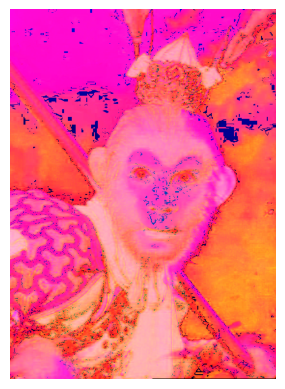
\includegraphics[width=\linewidth]{img/HSV.png}
		\caption{The original image in HSV color space.}
		\label{fig:hsv}
	\end{figure}
	
	\subsection{The classical Histogram Equalization}
	
	I applied the basic steps as in section 3, and Figure ~\ref{fig:HE} is the resulting image, and we can see that this image looks very sharp.
	
	\begin{figure}
		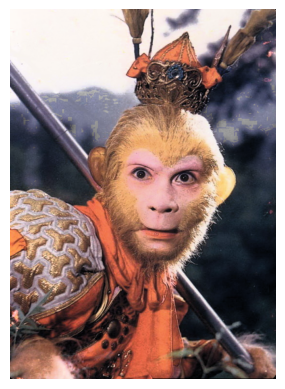
\includegraphics[width=\linewidth]{img/HE.png}
		\caption{The classical Histogram Equalization}
		\label{fig:HE}
	\end{figure}
	
	For more information Figure ~\ref{fig:original_histo} shows the original image histogram and Figure ~\ref{fig:original_cdf} shows the CDF calculated from the histogram:
	
	\begin{figure}
		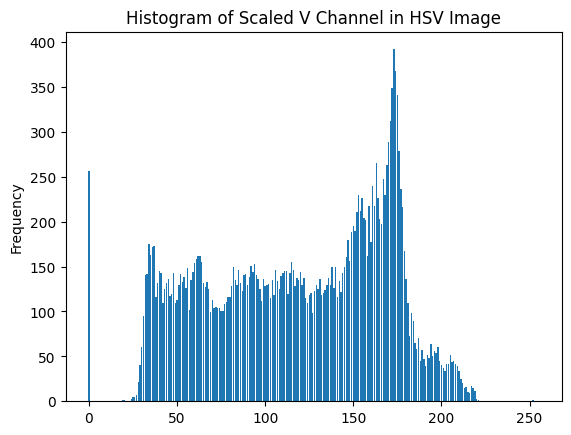
\includegraphics[width=\linewidth]{img/original_histo.png}
		\caption{The original histogram}
		\label{fig:original_histo}
	\end{figure}
	
	\begin{figure}
		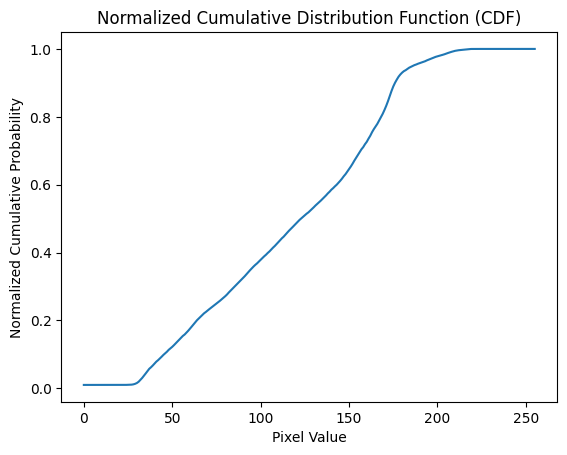
\includegraphics[width=\linewidth]{img/original_cdf.png}
		\caption{The original CDF}
		\label{fig:original_cdf}
	\end{figure}
	
	For this part, I tried to follow the coding style that you had shown us during the lecture week but I was still unable to follow it and needed to re-implement some kernel.
	
	\subsection{The Adjusted Histogram Equalization}
	
	For this part, I need to modify the original histogram to create a new histogram to make the histogram more uniform. The formula that I use to find the new histogram is shown in Figure ~\ref{fig:AHE_formula}.
	
	\begin{figure}[!h]
		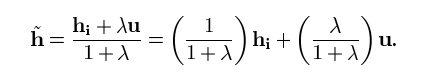
\includegraphics[width=\linewidth]{img/AHE_formula.PNG}
		\caption{The formula to find new histogram of AHE}
		\label{fig:AHE_formula}
	\end{figure}
	
	In which:
	\begin{itemize}
		\item hi is the input original histogram as in the previous part
		\item u is the uniform histogram where all the column in this histogram has equal value
		\item lamba is the parameter that we need to choose
	\end{itemize}
	
	For more information Figure ~\ref{fig:AHE_histo} shows the modified image histogram and Figure ~\ref{fig:AHE_cdf} shows the CDF calculated from this histogram. We can see that using AHE, the cdf now looks really like a straight line.
	
	\begin{figure}[!h]
		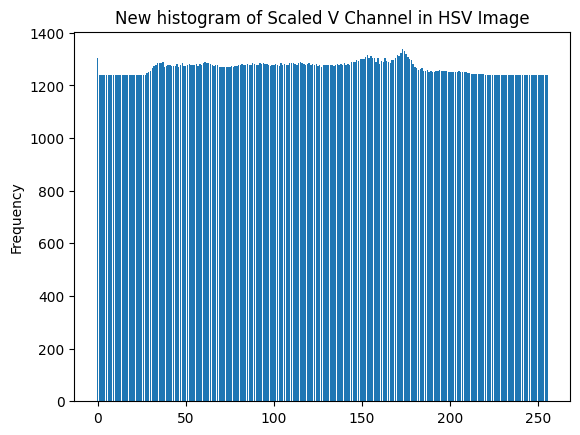
\includegraphics[width=\linewidth]{img/AHE_histo.png}
		\caption{The modified histogram}
		\label{fig:AHE_histo}
	\end{figure}
	
	\begin{figure}[!h]
		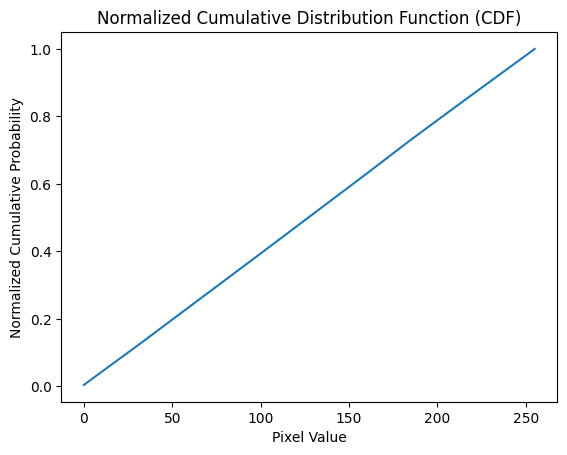
\includegraphics[width=\linewidth]{img/AHE_cdf.png}
		\caption{The new CDF}
		\label{fig:AHE_cdf}
	\end{figure}
	
	Figure ~\ref{fig:ahe_lamb_1}, Figure ~\ref{fig:ahe_lamb_3} and Figure ~\ref{fig:ahe_lamb_5} show the resulting image with lambda is 1, 3, 5 respectively.
	
	\begin{figure}[!h]
		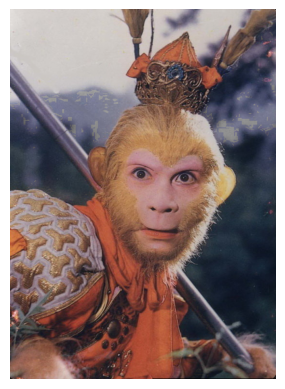
\includegraphics[width=\linewidth]{img/ahe_lamb_1.png}
		\caption{The AHE lambda 1}
		\label{fig:ahe_lamb_1}
	\end{figure}
	
	\begin{figure}[!h]
		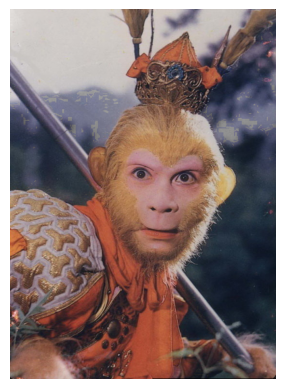
\includegraphics[width=\linewidth]{img/ahe_lamb_3.png}
		\caption{The AHE lambda 3}
		\label{fig:ahe_lamb_3}
	\end{figure}
	
	\begin{figure}[!h]
		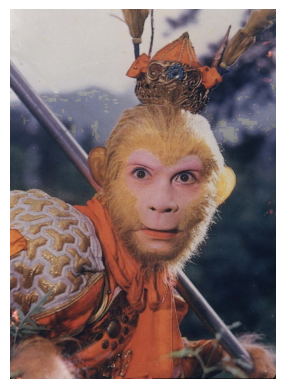
\includegraphics[width=\linewidth]{img/ahe_lamb_5.png}
		\caption{The AHE lambda 5}
		\label{fig:ahe_lamb_5}
	\end{figure}
	
	As you can see the image from this algorithm looks more natural compared to the classical one.
	
	\subsection{Weighted Histogram Equalization}
	
	For this part, I also need to modify the original histogram to create new histogram. The formula that I use to find the new histogram is shown in Figure ~\ref{fig:WHE_formula}.
	
	\begin{figure}[!h]
		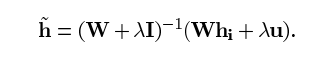
\includegraphics[width=\linewidth]{img/WHE_formula.PNG}
		\caption{The formula to find new histogram of WHE}
		\label{fig:WHE_formula}
	\end{figure}
	
	In which:
	\begin{itemize}
		\item W is the diagonal error weight matrix
		\item hi is the input original histogram as in the previous part
		\item u is the uniform histogram where all the column in this histogram has equal value
		\item lamba is the parameter that we need to choose
	\end{itemize}
	
	In this part, I have tried to figure out how to take an invert of a matrix using cuda and perform the multiplication but I wasn't successful in doing so, and overall in this part, I was only able to calculate the W matrix but still only in CPU and I also not sure that I is the correct one :(
	
	\subsection{EIHE}
	
	For this part, I follow the Algorithm ~\ref{alg:esihe} as stated in the paper in the bibliography of the project.
	
	\begin{algorithm}[H] % H means here
		\caption{ESIHE Algorithm}
		\label{alg:esihe}
		\begin{algorithmic}[1]
			\Require{A grayscale image $I$}
			\Ensure{A histogram-equalized image $J$}
			
			\State Compute the histogram $h(k)$ of $I$
			\State Compute the value of exposure and threshold parameter $x_a$
			\State Compute the clipping threshold $T_c$, and clip the histogram $h_c(k)$.
			\State Divide the clipped histogram into two sub-histograms using the threshold parameter $x_a$
			\State Apply the histogram equalization on individual sub-histograms.
			\State Combine the sub-images into one image $J$ for analysis
			
			\State \textbf{Return:} $J$
			
		\end{algorithmic}
	\end{algorithm}
	
	For more information Figure ~\ref{fig:EIHE_clipping_hist} shows the clipping histogram. And you can take a look at the notebook for other figures of this part
	
	\begin{figure}[!h]
		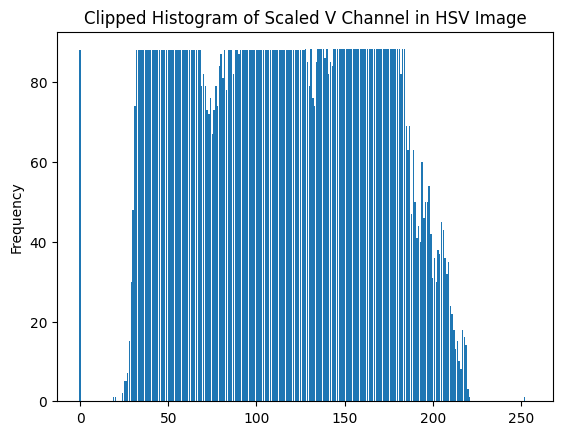
\includegraphics[width=\linewidth]{img/EIHE_clipping_hist.png}
		\caption{The clipping histogram of EIHE.}
		\label{fig:EIHE_clipping_hist}
	\end{figure}
	
	Figure ~\ref{fig:EIHE} is the resulting image, and we can see that this image shows some really weird parts and I think that I have made some mistakes in the implementation of it.
	
	\begin{figure}
		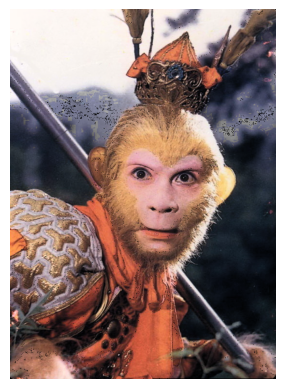
\includegraphics[width=\linewidth]{img/EIHE.png}
		\caption{The EIHE result.}
		\label{fig:EIHE}
	\end{figure}
	
	\section{Comparision}
	
	Table~\ref{tab:metric} shows the result of 2 metrics for these algorithms. The entropy is used to measure the content of an image, where a higher value indicates an image with richer details and the method with the highest entropy is EIHE and it is also the method that gives the most difference to the original image - through AME.
	
	\begin{center}
		\begin{tabular}{|c|c|c|c|}
			\hline
			& HE & AHE & EIHE \\ \hline
			AME & 56000788.0 & 56020416.0 & 58478404.0  \\ \hline
			Entropy & 7.4060 & 7.3808 & 7.5297  \\ \hline
			\label{tab:metric}
		\end{tabular}
	\end{center}
	
	Table~\ref{tab:time} shows the running time of the algorithms. This result is measured by running the file 5 times for each algorithm and taking the average result of them. 
	
	\begin{center}
		\begin{tabular}{|c|c|c|c|}
			\hline
			& HE & AHE & EIHE \\ \hline
			Running time & 2.7003s & 4.1533s & 7.645s \\ \hline
			\label{tab:time}
		\end{tabular}
	\end{center}
	
	\section{Conclusion}
	
	What I have done:
	\begin{itemize}
		\item Implementation of 3 algorithms HE, AHE and EIHE
		\item I tried to work with WHE but I can only find the W matrix
		\item All of the calculations are performed by Google Colaboratory
	\end{itemize}
	What is still missing and needs improvement:
	\begin{itemize}
		\item The code is not optimized and does not follow the format that you have shown us, I really need to reformat the code but it is too rushed for me :(
		\item There are still a lot of algorithms that I haven't implemented like WHE and I wasn't able to read about like MMSICHE, CLAHE, and ACLAHE
		\item The result of EIHE still has some weird parts.
	\end{itemize}
	
	Overall, I have tried my best with this project and I have been able to be more familiar with the concept of the course through this project.
	
\end{document}
